\documentclass[12pt, a4paper, brazil]{article}
\usepackage{fix-cm}

\usepackage[a4paper,
            top=3cm, bottom=2cm,
            left=3cm, right=2cm]{geometry}

\usepackage[num, overcite]{abntex2cite}
\citebrackets[]
\makeatletter
\renewcommand\@biblabel[1]{[#1] }
\makeatother

\usepackage{subcaption}
\usepackage{booktabs}
\usepackage{amsmath, amsfonts, amsthm, bm}
\usepackage{newtxtext, newtxmath, mathtools}
\usepackage[brazil]{babel}
\usepackage[T1]{fontenc}
\usepackage{indentfirst}
\usepackage{microtype}
\usepackage{fancyhdr}
\usepackage{graphicx}
\usepackage{ragged2e}
\usepackage{multirow}
\usepackage{multicol}
\usepackage{setspace}
\usepackage{icomma}
\usepackage{array}
\usepackage{float}
\usepackage{tikz}

\usepackage{silence}
\WarningFilter{latex}{Command \showhyphens has changed}

\onehalfspacing
\setlength{\parindent}{1.25cm}
\setlength{\parskip}{0.4\baselineskip}
\justifying

\usepackage{titlesec}

\newcommand{\titlefix}{
  \hyphenpenalty=10000
  \exhyphenpenalty=10000
  \emergencystretch=2em
}

\captionsetup{
    justification=centering
}

\titleformat{\section}
{\normalsize\bfseries\titlefix}
{\thesection.}
{0.5em}
{}

\titlespacing*{\section}
{0.75cm}
{1.5\baselineskip}
{0.8\baselineskip}

\titleformat{\subsection}
{\normalsize\bfseries\titlefix}
{\thesubsection.}
{0.5em}
{}

\titlespacing*{\subsection}
{1.5cm}
{1.2\baselineskip}
{0.6\baselineskip}

\titleformat{\subsubsection}
{\normalsize\bfseries\titlefix}
{\thesubsubsection.}
{0.5em}
{}

\titlespacing*{\subsubsection}
{2.25cm}
{1.0\baselineskip}
{0.4\baselineskip}

\titleformat{name=\section,numberless}
{\normalsize\bfseries\centering\titlefix}
{}
{0em}
{}

\titlespacing*{name=\section,numberless}
{0cm}
{1.5\baselineskip}
{0.8\baselineskip}

\newcounter{rownum}
\setcounter{rownum}{0}

\newcolumntype{N}{>{\stepcounter{rownum}\therownum.}l}

\begin{document}
\pagestyle{empty}

\begin{center}

	
\includegraphics[width=0.3\textwidth]{ita_rgb.jpg}

	\vfill

	{\large\bfseries
		Variáveis Contínuas e Distribuição Gaussiana\\[2.0\baselineskip]
	}

	\vfill

	{\normalsize\bfseries
		Caio Schaden Ishida\\[0.5\baselineskip]
		Felipe Osternes da Silva\\[0.5\baselineskip]
		João Victor Evers Cordeiro\\[0.5\baselineskip]
		Paulo Vinícius Rodrigues Azevedo\\[0.5\baselineskip]
		Rafael Sakata Suzuki\\[0.5\baselineskip]
	}

	\vfill

	{\normalsize\bfseries
		Grupo nº 01\\[0.6\baselineskip]
		Turma 30.2
	}

	\vfill

	{\normalsize
		\textbf{Professores}\\[0.5\baselineskip]
		Prof. Marco Antonio Ridenti (coord.)\\
		Prof. Amós Silva\\
		Profa. Sônia Guimarães\\
		Prof. Filipe Matusalém\\
		Prof. Bogos Sismanoglu\\[0.5\baselineskip]
		Data de entrega: 27/08/2026
	}

	\vfill

	{\normalsize\bfseries
		Departamento de Física\\
		Divisão de Ciências Fundamentais\\
		Instituto Tecnológico de Aeronáutica - ITA
	}

\end{center}

\newpage

\pagestyle{fancy}
\fancyhf{}
\fancyfoot[R]{\thepage}
\renewcommand{\headrulewidth}{0pt}
\setcounter{page}{1}

\section{OBJETIVOS}
O objetivo principal deste experimento foi determinar um valor para a aceleração da gravidade local a partir
do modelo teórico de um pêndulo simples, cujo período de oscilação é dado por $2\pi\sqrt{\frac{l}{g}}$. Para
isso, foram realizadas repetidas medições do período do pêndulo utilizando diferentes instrumentos, de modo a
avaliar a influência das medições experimentais sobre o valor obtido para $g$. Os resultados foram então
comparados com um valor de referência para a aceleração da gravidade local. Além disso, buscou-se analisar
a distribuição das frequências dos valores medidos e verificar sua compatibilidade com uma distribuição de
probabilidade Gaussiana.

\newpage
\section{PROCEDIMENTO EXPERIMENTAL}
Para cumprir o objetivo traçado minimizando as incertezas relativas, foram realizadas 100 medições do período de oscilação de um pêndulo simples composto
por uma massa esférica presa a um suporte por um fio, totalizando em uma distância entre o centro de massa e o apoio no suporte de $l= (35,00\pm0,05)\ \text{cm}$,
como mostra a Figura \ref{fig:pendulo}.

\begin{figure}[H]
	\centering
	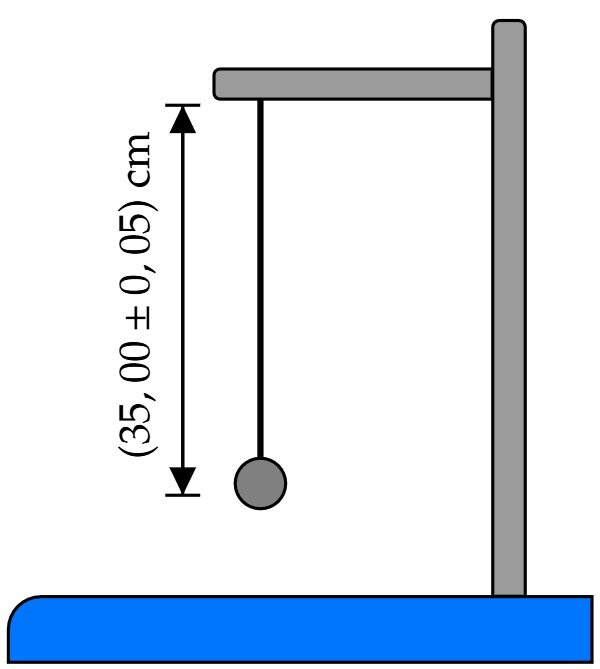
\includegraphics[width=0.45\linewidth]{pendulo.jpeg}
	\caption{Arranjo experimental utilizado para a determinação da gravidade}
	\label{fig:pendulo}
\end{figure}



\section{RESULTADOS}
A Tabela \ref{tab:medições}
contém as medições  do período de oscilação do pêndulo utilizando um cronômetro.
\begin{table}[H]
	\centering
	\caption{Medições do período de oscilação do pêndulo ($T$) em segundos.}
	\label{tab:medições}
	\vspace{0.5\baselineskip}
	\begin{tabular}{r l @{\hspace{0.8cm}} r l @{\hspace{0.8cm}} r l @{\hspace{0.8cm}} r l}
		\hline
		\multicolumn{1}{c}{nº} & \multicolumn{1}{c}{$T$ (s)} & \multicolumn{1}{c}{nº} & \multicolumn{1}{c}{$T$ (s)} & \multicolumn{1}{c}{nº} & \multicolumn{1}{c}{$T$ (s)} & \multicolumn{1}{c}{nº} & \multicolumn{1}{c}{$T$ (s)} \\
		\hline
		1.                     & 1,1925000                   & 26.                    & 1,1915000                   & 51.                    & 1,1911000                   & 76.                    & 1,1898000                   \\
		2.                     & 1,1920000                   & 27.                    & 1,1917000                   & 52.                    & 1,1905000                   & 77.                    & 1,1896000                   \\
		3.                     & 1,1922000                   & 28.                    & 1,1915000                   & 53.                    & 1,1910000                   & 78.                    & 1,1904000                   \\
		4.                     & 1,1910000                   & 29.                    & 1,1912000                   & 54.                    & 1,1906000                   & 79.                    & 1,1896000                   \\
		5.                     & 1,1934000                   & 30.                    & 1,1918000                   & 55.                    & 1,1910000                   & 80.                    & 1,1901000                   \\
		6.                     & 1,1928000                   & 31.                    & 1,1913000                   & 56.                    & 1,1902000                   & 81.                    & 1,1896000                   \\
		7.                     & 1,1923000                   & 32.                    & 1,1916000                   & 57.                    & 1,1903000                   & 82.                    & 1,1894000                   \\
		8.                     & 1,1921000                   & 33.                    & 1,1915000                   & 58.                    & 1,1904000                   & 83.                    & 1,1896000                   \\
		9.                     & 1,1922000                   & 34.                    & 1,1911000                   & 59.                    & 1,1903000                   & 84.                    & 1,1905000                   \\
		10.                    & 1,1920000                   & 35.                    & 1,1917000                   & 60.                    & 1,1906000                   & 85.                    & 1,1898000                   \\
		11.                    & 1,1918000                   & 36.                    & 1,1910000                   & 61.                    & 1,1909000                   & 86.                    & 1,1891000                   \\
		12.                    & 1,1920000                   & 37.                    & 1,1910000                   & 62.                    & 1,1904000                   & 87.                    & 1,1906000                   \\
		13.                    & 1,1919000                   & 38.                    & 1,1907000                   & 63.                    & 1,1902000                   & 88.                    & 1,1895000                   \\
		14.                    & 1,1925000                   & 39.                    & 1,1910000                   & 64.                    & 1,1904000                   & 89.                    & 1,1905000                   \\
		15.                    & 1,1909000                   & 40.                    & 1,1906000                   & 65.                    & 1,1906000                   & 90.                    & 1,1895000                   \\
		16.                    & 1,1918000                   & 41.                    & 1,1905000                   & 66.                    & 1,1900000                   & 91.                    & 1,1899000                   \\
		17.                    & 1,1919000                   & 42.                    & 1,1906000                   & 67.                    & 1,1904000                   & 92.                    & 1,1904000                   \\
		18.                    & 1,1921000                   & 43.                    & 1,1908000                   & 68.                    & 1,1901000                   & 93.                    & 1,1900000                   \\
		19.                    & 1,1917000                   & 44.                    & 1,1905000                   & 69.                    & 1,1902000                   & 94.                    & 1,1898000                   \\
		20.                    & 1,1920000                   & 45.                    & 1,1905000                   & 70.                    & 1,1901000                   & 95.                    & 1,1904000                   \\
		21.                    & 1,1918000                   & 46.                    & 1,1903000                   & 71.                    & 1,1903000                   & 96.                    & 1,1899000                   \\
		22.                    & 1,1919000                   & 47.                    & 1,1907000                   & 72.                    & 1,1897000                   & 97.                    & 1,1898000                   \\
		23.                    & 1,1913000                   & 48.                    & 1,1908000                   & 73.                    & 1,1909000                   & 98.                    & 1,1899000                   \\
		24.                    & 1,1917000                   & 49.                    & 1,1904000                   & 74.                    & 1,1899000                   & 99.                    & 1,1899000                   \\
		25.                    & 1,1921000                   & 50.                    & 1,1901000                   & 75.                    & 1,1906000                   & 100.                   & 1,1895000                   \\
		\hline
	\end{tabular}
\end{table}
\end{table}


A Tabela \ref{tab:resultados} contém os valores e incertezas finais dos períodos medidos utilizando cronômetro de mão ($T^{(1)}$) e de bancada ($T^{(2)}$), as estimativas obtidas da aceleração da gravidade local ($g^{(1)}$ e $g^{(2)}$, respectivamente), e o valor de referência da aceleração local da gravidade $g_{0}$

\begin{table}[H]
	\centering
	\caption{Valores e incertezas finais dos períodos medidos utilizando cronômetro de mão ($T^{(1)}$) e de bancada ($T^{(2)}$), as estimativas experimentais da aceleração da gravidade local associadas ($g^{(1)}$ e $g^{(2)}$, respectivamente), e o valor de referência da aceleração local da gravidade $g_{0}$}
	\begin{tabular}{l l l}
		\hline
		Grandeza                    & Valor   & Incerteza \\[0.5ex]
		\hline
		$T\ \mathrm{(s)}$           & $1,174$ & 0,012     \\
		$g \mathrm{(m/s^{2})}$      & $10,03$ & 0,15      \\
		$g_{0}\ \mathrm{(m/s^{2})}$ & $9,786$ &           \\
		\hline
	\end{tabular}
	\label{tab:resultados}
\end{table}

Por fim, a Figura \ref{fig:histogramas} contém os histogramas dos valores medidos para os cronômetros de mesa e bancada comparados aos valores teóricos esperados para uma distribuição Gaussiana com desvios padrão calculados por meio de .

\begin{figure}[H]
	\centering
	\caption{Histograma de frequência das medidas}
	\label{fig:histogramas}

\end{figure}

\newpage
\section{DISCUSSÃO}

\begin{equation}\label{eq:comp}
	q = \frac{\sum_{i}(f_{Gauss,i}-{f_{hist}})^2}{\sum_{i}(f_{hist, i}-\overline{f_{hist}})^2}
\end{equation}

Nesse cálculo, o coeficiente $q$ assume valor nulo se a distribuição ajusta perfeitamente os dados experimentais obtidos, enquanto seu valor se distancia de $0$ quando a distribuição proposta não ajusta bem os dados.

A Figura \ref{fig:desvios} é uma representação gráfica para os desvios da distribuição Gaussiana em relação às observações experimentais para cada um dos cronômetros, dados por $\delta = f_{Gauss} - f_{hist}$.


\newpage

\clearpage
\renewcommand{\refname}{}
\section{REFERÊNCIAS}
\vspace{-1.5\baselineskip}
\bibliography{referencias_sintese3}

\end{document}
